\chapter{Fonctions d’onde de l’oscillateur, spin un demi et échange de particules}

\section{Des oscillateurs partout}

Tout système possédant un équilibre stable peut osciller lorsqu’on l’en écarte. Il peut avoir une seule fréquence ou plusieurs. Une corde de violon, par exemple, possède un mode fondamental et des harmoniques supérieures. La pincer excite une certaine combinaison de ces modes.

Les exemples les plus importants ici sont les champs. La configuration d’équilibre du champ électromagnétique est le vide : pas de champ électrique, pas de champ magnétique et pas d’oscillation électromagnétique. Si l’on introduit un rayonnement dans une cavité ou un guide d’ondes, le champ peut osciller selon ses modes permis, chacun ayant sa propre fréquence. Dans la théorie quantique, ces modes décrivent des ensembles de photons.

La même idée s’applique à un cristal. Il est trompeur de se représenter chaque atome comme un oscillateur indépendant. Les atomes exercent des forces les uns sur les autres, si bien que le déplacement d’un atome affecte ses voisins et qu’une onde se propage dans le cristal. Les modes normaux de ce mouvement couplé sont des oscillateurs harmoniques, et leurs quanta sont appelés phonons. Photons et phonons sont des objets physiques différents, mais tous deux ramènent à la même algèbre de l’oscillateur.

\section{L’algèbre de l’oscillateur}

Pour étudier l’oscillateur, posons la masse et la constante de Planck réduite égales à un :
\[
m=1,\qquad \hbar=1.
\]
Le Hamiltonien est
\begin{equation}
H=\frac{p^{2}}{2}+\frac{\omega^{2}x^{2}}{2}.
\end{equation}
Le paramètre \(\omega\) fixe la courbure du potentiel et correspond aussi à la fréquence d’oscillation.

Définissons les opérateurs de montée et de descente par
\begin{equation}
A_{\pm}=\frac{p\pm i\omega x}{\sqrt{2\omega}}.
\end{equation}
La normalisation est choisie de sorte que
\begin{equation}
[A_{-},A_{+}]=1.
\end{equation}
L’opérateur nombre est
\begin{equation}
N=A_{+}A_{-}.
\end{equation}
Ensemble, ces équations impliquent que \(A_{+}\) augmente d’une unité une valeur propre de \(N\) et que \(A_{-}\) la diminue d’une unité. Le spectre qui en résulte est
\begin{equation}
n=0,1,2,3,\ldots .
\end{equation}

Le produit des deux opérateurs d’échelle fait aussi apparaître la correction quantique à l’énergie classique :
\begin{align}
N
&=\frac{1}{2\omega}(p+i\omega x)(p-i\omega x)\\
&=\frac{1}{2\omega}\left(p^{2}+\omega^{2}x^{2}
 +i\omega[x,p]\right)\\
&=\frac{1}{2\omega}\left(p^{2}+\omega^{2}x^{2}-\omega\right),
\end{align}
où \([x,p]=i\). Par conséquent,
\begin{equation}
H=\omega\left(N+\frac12\right).
\end{equation}
Si la constante additive n’a pas d’importance pour le problème, il est commode d’utiliser le Hamiltonien décalé
\begin{equation}
H_{\mathrm{shifted}}=H-\frac{\omega}{2}=\omega N.
\end{equation}
Le terme \(\omega/2\) est l’énergie de point zéro, ou énergie de l’état fondamental, de l’oscillateur. Pour un mode de champ, le terme analogue est appelé énergie du vide. Il reflète le principe d’incertitude : aucun état ne peut avoir à la fois \(x\) et \(p\) exactement égaux à zéro, si bien que les deux termes quadratiques positifs dans \(H\) ne peuvent pas avoir tous deux une valeur moyenne nulle.

\begin{classroomqa}
\lecturetimestamp{00:09:46}
\audiencequestion{Pourquoi zéro fait-il partie du spectre de l’opérateur nombre ?}
\lecturerresponse{On peut le démontrer explicitement en construisant la fonction d’onde de l’état fondamental. Cette construction fera apparaître un état tel que \(N=0\).}
\end{classroomqa}

Pour commencer cette construction, remplaçons les vecteurs d’état par des fonctions d’onde de position. Les états propres de l’énergie deviennent
\[
\psi_{0}(x),\ \psi_{1}(x),\ \psi_{2}(x),\ldots,
\]
et les opérateurs fondamentaux agissent comme suit :
\begin{equation}
X\longmapsto x,\qquad
P\longmapsto -i\frac{d}{dx}.
\end{equation}
En rétablissant \(\hbar\), le second remplacement serait
\(P\mapsto-i\hbar\,d/dx\).

Avant de résoudre l’équation pour \(\psi_{0}\), on peut répondre plus rapidement à la question par un raisonnement abstrait. Sur l’échelle discrète des états propres normalisables de l’oscillateur, \(N=A_{+}A_{-}\) est non négatif ; des abaissements répétés par unités ne peuvent donc pas se poursuivre indéfiniment. À l’extrémité---dont on construira plus bas la fonction d’onde normalisable---il doit exister un état, noté \(\lvert0\rangle\), tel que
\begin{equation}
A_{-}\lvert0\rangle=\mathbf 0.
\end{equation}
Sinon, \(A_{-}\lvert0\rangle\) serait un autre état, situé une unité plus bas. Il s’ensuit immédiatement que
\begin{equation}
N\lvert0\rangle
=A_{+}A_{-}\lvert0\rangle
=\mathbf 0
=0\,\lvert0\rangle.
\end{equation}
L’état le plus bas a donc pour valeur propre de nombre zéro.

\begin{classroomqa}
\lecturetimestamp{00:14:57}
\audiencequestion{Si la valeur propre est zéro, le membre de droite ne devrait-il pas contenir un vecteur propre nul ?}
\lecturerresponse{Le ket \(\lvert0\rangle\) est un vecteur normalisé non nul dont l’étiquette est zéro. Dans \(N\lvert0\rangle=0\,\lvert0\rangle\), le membre de droite est le vecteur nul. Le ket de l’état fondamental et le vecteur nul sont des objets différents.}
\end{classroomqa}

\section{L’équation de Schr\"odinger et les solutions physiques}

Revenons maintenant à la représentation de position. L’équation de Schr\"odinger indépendante du temps est
\begin{equation}
\left[
-\frac12\frac{d^{2}}{dx^{2}}
+\frac12\omega^{2}x^{2}
\right]\psi(x)=E\psi(x).
\end{equation}
En tant qu’équation différentielle du second ordre, elle possède des solutions formelles pour des valeurs arbitraires de \(E\). La plupart de ces solutions formelles ne correspondent pas à des états physiques de l’oscillateur. Elles croissent exponentiellement lorsque \(\lvert x\rvert\) devient grand, si bien que leur norme diverge.

Pour un état lié, la fonction d’onde doit être de carré intégrable :
\begin{equation}
\int_{-\infty}^{\infty}\psi^{*}(x)\psi(x)\,dx<\infty.
\end{equation}
On peut alors la normaliser de sorte que l’intégrale soit égale à un. Seules certaines valeurs particulières de l’énergie donnent de telles solutions. À cet égard, les états de position et de quantité de mouvement sur une droite infinie font exception, mais les solutions de l’oscillateur qui croissent exponentiellement sont tout simplement exclues de l’espace des états.

\section{L’état fondamental gaussien}

On peut résoudre l’équation du second ordre, mais l’algèbre des opérateurs d’échelle donne une équation du premier ordre plus simple :
\begin{equation}
A_{-}\psi_{0}(x)=0.
\end{equation}
Le facteur global dans \(A_{-}\) n’a pas d’importance lorsque le membre de droite est nul ; cette équation équivaut donc à
\begin{equation}
(p-i\omega x)\psi_{0}(x)=0.
\end{equation}
En utilisant \(p=-i\,d/dx\), on obtient
\begin{equation}
\left(\frac{d}{dx}+\omega x\right)\psi_{0}(x)=0.
\end{equation}

\begin{classroomqa}
\lecturetimestamp{00:22:32}
\audiencequestion{Peut-on résoudre cette équation par séparation des variables ?}
\lecturerresponse{Il n’y a qu’une variable indépendante ; il n’y a donc pas deux variables à séparer. Écrite sous la forme \(\psi_{0}'/\psi_{0}=-\omega x\), l’équation ressemble à une dérivée logarithmique. Cela suggère d’écrire la fonction d’onde sous forme exponentielle.}
\end{classroomqa}

Une méthode utile consiste à poser
\begin{equation}
\psi_{0}(x)=e^{f(x)}.
\end{equation}
Alors
\[
\psi_{0}'(x)=f'(x)e^{f(x)},
\]
et le facteur exponentiel commun se simplifie. L’équation se réduit à
\begin{equation}
\frac{df}{dx}+\omega x=0.
\end{equation}

\begin{classroomqa}
\lecturetimestamp{00:26:28}
\audiencequestion{Ne devrait-il pas y avoir un signe moins dans \(f(x)\) ?}
\lecturerresponse{Oui. Puisque \(df/dx=-\omega x\), l’intégration donne un terme quadratique négatif.}
\end{classroomqa}

On a donc
\begin{equation}
f(x)=-\frac12\omega x^{2}+C,
\end{equation}
et
\begin{equation}
\psi_{0}(x)\propto e^{-\omega x^{2}/2}.
\end{equation}
La constante multiplicative de normalisation n’est pas précisée. L’essentiel est la forme gaussienne : la fonction est lisse, concentrée près de l’origine et décroît rapidement lorsque \(\lvert x\rvert\) devient grand. Elle est manifestement de carré intégrable.

Il n’est pas nécessaire de réinjecter la réponse dans l’équation du second ordre pour trouver son énergie. L’algèbre donne déjà
\begin{equation}
E_{0}=\frac{\omega}{2}.
\end{equation}

\section{États excités, nœuds et mouvement classique}

Le premier état excité s’obtient en appliquant l’opérateur de montée à l’état fondamental :
\begin{equation}
\psi_{1}(x)\propto A_{+}\psi_{0}(x)
\propto(p+i\omega x)e^{-\omega x^{2}/2}.
\end{equation}
L’équation de l’état fondamental indique que
\[
p\psi_{0}=i\omega x\,\psi_{0}.
\]
Le changement de signe dans l’opérateur d’échelle transforme la soustraction en addition :
\begin{equation}
(p+i\omega x)\psi_{0}
=2i\omega x\,\psi_{0}.
\end{equation}
À une constante globale près,
\begin{equation}
\psi_{1}(x)\propto x\,e^{-\omega x^{2}/2}.
\end{equation}

Cette fonction d’onde est impaire :
\begin{equation}
\psi_{1}(-x)=-\psi_{1}(x).
\end{equation}
Sa densité de probabilité est paire, mais elle possède un nœud à l’origine,
\begin{equation}
\lvert\psi_{1}(0)\rvert^{2}=0.
\end{equation}
La densité de probabilité du premier état excité possède donc un nœud en \(x=0\).

Des applications répétées de \(A_{+}\) donnent des polynômes de degré croissant multipliant la même enveloppe gaussienne.\footnote{Le cours indique les facteurs polynomiaux de degré supérieur, le nœud supplémentaire à chaque étape et l’alternance de parité de \(00{:}34{:}25\) à \(00{:}35{:}49\). La forme produit d’une gaussienne par un polynôme est confirmée par la discussion des fonctions propres de l’oscillateur dans l’ouvrage de Leonard Susskind et Art Friedman, \emph{Quantum Mechanics: The Theoretical Minimum} (2014).}À un facteur de normalisation près,
\begin{equation}
\psi_{n}(x)=P_{n}(x)e^{-\omega x^{2}/2}.
\end{equation}
La parité alterne entre paire et impaire, et chaque étape ajoute un nœud. Lorsque \(n\) augmente, la fonction d’onde s’étend plus loin de l’origine et ses oscillations deviennent plus rapides.

Ces deux caractéristiques ont des significations physiques directes. Une fonction d’onde qui s’étend plus loin de l’origine correspond à une énergie potentielle plus élevée, car le potentiel croît comme \(x^{2}\). Des oscillations rapides dans l’espace des positions signalent une quantité de mouvement plus grande. Un oscillateur fortement excité a tendance à s’éloigner davantage du centre ; lorsqu’il traverse la région centrale, sa quantité de mouvement est plus grande et sa fonction d’onde y oscille plus rapidement.

\begin{classroomqa}
\lecturetimestamp{00:37:18}
\audiencequestion{L’oscillateur harmonique cesse-t-il de se rapprocher du comportement classique lorsque \(n\) devient grand ?}
\lecturerresponse{Le mouvement classique n’est pas représenté par un seul état propre stationnaire de l’énergie. Il apparaît dans un paquet d’ondes qui contient plusieurs niveaux d’énergie. Une gaussienne déplacée, par exemple, évolue en oscillant comme un oscillateur classique, et l’incertitude relative diminue à mesure que l’amplitude de l’oscillation augmente.}
\end{classroomqa}

Partons de la gaussienne de l’état fondamental et déplaçons-la par rapport à l’origine. Le paquet ainsi déplacé n’est plus un état propre de l’énergie ; c’est une superposition de nombreux états propres. Selon l’équation de Schr\"odinger dépendante du temps, ses composantes acquièrent des phases différentes. Le paquet oscille d’un côté à l’autre du potentiel, présentant de rapides variations de phase près du centre et redevenant lisse près d’un point de retournement. Plus l’excursion est grande devant la largeur du paquet, plus le mouvement paraît classique.

\begin{classroomqa}
\lecturetimestamp{00:39:29}
\audiencequestion{La fonction d’onde du deuxième état excité devrait-elle s’annuler à l’origine ?}
\lecturerresponse{Non. Son facteur polynomial n’est pas simplement \(x^{2}\) ; il contient aussi un terme constant, de sorte que la fonction d’onde n’a pas nécessairement à s’annuler en \(x=0\).}
\end{classroomqa}

Le raisonnement par opérateurs d’échelle suppose aussi que \(A_{+}\) et \(A_{-}\) sont adjoints l’un de l’autre sur le domaine des fonctions de l’oscillateur de carré intégrable, avec le comportement aux limites requis pour la relation d’adjonction. Les solutions formelles qui croissent exponentiellement n’appartiennent pas à ce domaine.

\begin{classroomqa}
\lecturetimestamp{00:40:45}
\audiencequestion{Existe-t-il un moyen général de reconnaître les Hamiltoniens que l’on peut résoudre par ces méthodes algébriques ?}
\lecturerresponse{Il n’existe pas de règle générale de ce type. Les exemples exactement solubles sont rares. L’oscillateur harmonique et l’atome d’hydrogène idéal non relativiste sont des cas heureux où les méthodes algébriques fonctionnent.}
\end{classroomqa}

\section{Le spin un demi comme moment cinétique}

Le spin est un moment cinétique porté par une particule indépendamment de son mouvement orbital autour de son centre de masse. Une particule au repos n’a pas de moment cinétique orbital \(\mathbf R\times\mathbf P\), mais elle peut tout de même avoir un spin. On peut essayer de se représenter un minuscule objet en rotation, ou traiter le spin comme une propriété quantique intrinsèque. L’affirmation décisive est mathématique : ses composantes se transforment sous les rotations spatiales et obéissent aux relations de commutation du moment cinétique.

Rétablissons \(\hbar\) à partir d’ici. Les composantes du moment cinétique vérifient
\begin{equation}
[L_{z},L_{x}]=i\hbar L_{y},
\end{equation}
les deux autres relations s’obtenant par permutation cyclique. Les matrices de Pauli sans dimension sont
\begin{equation}
\begin{aligned}
\sigma_{z}&=
\begin{pmatrix}
1&0\\
0&-1
\end{pmatrix},\\[0.4em]
\sigma_{x}&=
\begin{pmatrix}
0&1\\
1&0
\end{pmatrix},\\[0.4em]
\sigma_{y}&=
\begin{pmatrix}
0&-i\\
i&0
\end{pmatrix}.
\end{aligned}
\end{equation}
Dans cette base, \(\sigma_{z}\) est diagonale. Ses valeurs propres sont \(+1\) et
\(-1\).

\begin{classroomqa}
\lecturetimestamp{00:47:35}
\audiencequestion{Y a-t-il un signe moins dans \(\sigma_x\) ?}
\lecturerresponse{Non. Les deux éléments hors diagonale de \(\sigma_x\) sont positifs.}
\end{classroomqa}

Le calcul au tableau à \(00{:}49{:}35\) commence le produit terme à terme. En terminant les produits, on obtient
\begin{align}
\sigma_{z}\sigma_{x}
&=
\begin{pmatrix}
0&1\\
-1&0
\end{pmatrix}
=i\sigma_{y},\\
\sigma_{x}\sigma_{z}
&=
\begin{pmatrix}
0&-1\\
1&0
\end{pmatrix}
=-i\sigma_{y}.
\end{align}
Il s’ensuit que
\begin{equation}
[\sigma_{z},\sigma_{x}]=2i\sigma_{y}.
\end{equation}
On élimine le facteur deux supplémentaire en définissant les opérateurs de spin physiques comme suit :\footnote{Le calcul au tableau omet \(\hbar\). Il est rétabli ici afin que \(S_i\) ait les unités d’un moment cinétique.}
\begin{equation}
S_{i}=\frac{\hbar}{2}\sigma_{i}.
\end{equation}
On a alors
\begin{equation}
[S_{z},S_{x}]=i\hbar S_{y},
\end{equation}
et de même pour les permutations cycliques. La moitié des matrices de Pauli, avec le facteur \(\hbar\) rétabli, forme donc un système de moment cinétique.

En posant \(\hbar=1\), on obtient la forme présentée ci-dessous.\footnote{La séquence source est \texttt{lecture\_04\_frame\_02.png}.}
\begin{figure}[htbp]
\centering
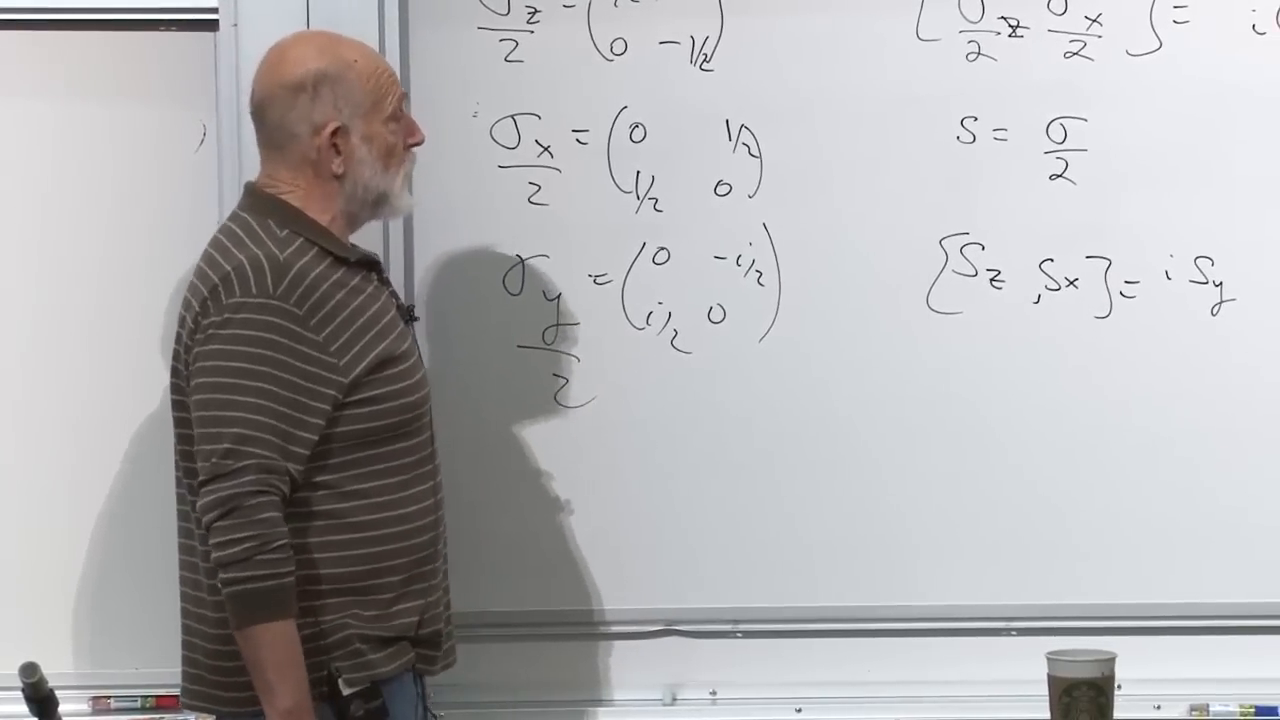
\includegraphics[width=0.9\linewidth]{lecture_04_frame_02.png}
\caption{En unités où \(\hbar=1\), la moitié des matrices de Pauli correspond aux opérateurs de moment cinétique de spin un demi et vérifie \([S_z,S_x]=iS_y\).}
\lectureframe{00:55:41}
\end{figure}

Les deux équations aux valeurs propres de \(S_z\) sont
\begin{equation}
S_z\lvert\pm\rangle
=\pm\frac{\hbar}{2}\lvert\pm\rangle.
\end{equation}
De manière équivalente, le nombre quantique magnétique sans dimension est
\begin{equation}
m_{s}=\pm\frac12,
\qquad
S_{z}\lvert m_{s}\rangle
=m_{s}\hbar\,\lvert m_{s}\rangle.
\end{equation}
Les opérateurs de montée et de descente du moment cinétique décalent \(m\) par pas entiers, mais cela n’implique pas que chaque échelle passe par zéro. Les multiplets de spin entier contiennent des valeurs entières de \(m\), tandis que ceux de spin demi-entier contiennent des valeurs demi-entières. Pour le spin un demi, l’échelle ne comporte que les deux états \(m_s=+1/2\) et \(m_s=-1/2\).

Ces deux états forment le doublet de spin un demi. Les électrons, les muons, les neutrinos et les quarks font partie des particules décrites par de tels multiplets de spin demi-entier.

\section{Moment cinétique orbital et spin}

Il existe maintenant deux types de moment cinétique. Le moment cinétique orbital décrit le mouvement par rapport à une origine,
\begin{equation}
\mathbf L=\mathbf R\times\mathbf P,
\end{equation}
tandis que \(\mathbf S\) est le spin intrinsèque. Leur somme vectorielle est le moment cinétique total,
\begin{equation}
\mathbf J=\mathbf L+\mathbf S.
\end{equation}

\begin{classroomqa}
\lecturetimestamp{00:56:49}
\audiencequestion{Si un système a un moment cinétique total \(\mathbf J\), comment détermine-t-on son spin \(\mathbf S\) ?}
\lecturerresponse{Les nombres quantiques de spin et de moment cinétique orbital sont normalement fournis séparément. Si \(L=0\), tout le moment cinétique est du spin. Sinon, il faut les règles quantiques d’addition des moments cinétiques, qui seront présentées plus tard.}
\end{classroomqa}

Les règles d’addition s’appliquent aussi bien à la somme du moment cinétique orbital et du spin qu’à deux spins ou à deux moments cinétiques orbitaux. Le système composé possède ses propres valeurs permises du moment cinétique total, mais ces règles ne sont pas encore nécessaires.

\begin{classroomqa}
\lecturetimestamp{00:58:18}
\audiencequestion{Quelles observations expérimentales ont conduit à introduire le spin ?}
\lecturerresponse{La spectroscopie en a fourni des indices, mais le tableau périodique donne une motivation particulièrement claire : sa structure en couches exige que les électrons possèdent une propriété supplémentaire à deux valeurs.}
\end{classroomqa}

\section{Dégénérescence hydrogénoïde et dénombrement des couches}

Pour le moment cinétique orbital, l’équation aux valeurs propres de \(L^{2}\) est
\begin{equation}
L^{2}\lvert\ell,m\rangle
=\hbar^{2}\ell(\ell+1)\lvert\ell,m\rangle,
\end{equation}
et une valeur fixée de \(\ell\) possède
\begin{equation}
2\ell+1
\end{equation}
états magnétiques, correspondant à \(m=-\ell,-\ell+1,\ldots,\ell\).

Le problème coulombien idéal non relativiste présente une dégénérescence supplémentaire. Les énergies des états liés sont négatives et tendent vers zéro par valeurs négatives, mais seul l’alignement des niveaux importe ici pour le dénombrement. Le premier niveau \(\ell=1\) est aligné sur le niveau \(\ell=0\) suivant ; le premier niveau \(\ell=2\) rejoint la couche principale suivante, et le motif se poursuit.\footnote{\texttt{lecture\_04\_frame\_03.png}, \(01{:}02{:}01\) ; l’alignement complet des couches principales est énoncé de \(01{:}02{:}33\) à \(01{:}04{:}10\).}

\begin{figure}[htbp]
\centering
\begin{tikzpicture}[x=1.55cm,y=1.0cm]
\draw[->] (-0.65,0) -- (-0.65,4.35);
\draw[->] (-0.85,0) -- (4.75,0);
\node at (-0.95,4.08) {\(E\)};
\node at (4.55,-0.28) {\(\ell\)};
\node at (0,-0.30) {\(0\)};
\node at (2,-0.30) {\(1\)};
\node at (4,-0.30) {\(2\)};

\draw (-0.20,0.75) -- (0.20,0.75);

\draw (-0.20,2.00) -- (0.20,2.00);
\foreach \dx in {-0.18,0,0.18}
  \draw (2+\dx-0.06,2.00) -- (2+\dx+0.06,2.00);

\draw (-0.20,3.15) -- (0.20,3.15);
\foreach \dx in {-0.18,0,0.18}
  \draw (2+\dx-0.06,3.15) -- (2+\dx+0.06,3.15);
\foreach \dx in {-0.32,-0.16,0,0.16,0.32}
  \draw (4+\dx-0.05,3.15) -- (4+\dx+0.05,3.15);

\node[anchor=west] at (0.35,0.75) {\(n=1\)};
\node[anchor=west] at (2.35,2.00) {\(n=2\)};
\node[anchor=west] at (4.40,3.15) {\(n=3\)};
\end{tikzpicture}
\caption{Les trois premières couches coulombiennes idéales regroupent des multiplets orbitaux de même énergie principale : un état dans la première couche, \(1+3\) dans la deuxième et \(1+3+5\) dans la troisième.}
\lectureframe{01:02:01}
\end{figure}

Dans la couche principale \(n\), les valeurs orbitales permises sont\footnote{Cette plage compacte de valeurs de \(\ell\) et la somme ci-dessous reconstituent les alignements de niveaux et les nombres d’états \(1,4,9,16,\ldots\) indiqués de \(01{:}02{:}33\) à \(01{:}04{:}10\). Le début du diagramme de spectre apparaît dans \texttt{lecture\_04\_frame\_03.png} à \(01{:}02{:}01\).}
\[
\ell=0,1,\ldots,n-1.
\]
Le nombre d’états spatiaux est donc
\begin{equation}
\sum_{\ell=0}^{n-1}(2\ell+1)=n^{2},
\end{equation}
ce qui donne la suite
\begin{equation}
1,\ 4,\ 9,\ 16,\ldots .
\end{equation}
Ce dénombrement ne porte que sur les états spatiaux. Chaque état spatial admet deux valeurs de spin ; les nombres totaux correspondants dans ce modèle idéal sont donc
\begin{equation}
2,\ 8,\ 18,\ 32,\ldots=2n^{2}.
\end{equation}

\section{Exclusion et propriété électronique à deux valeurs}

Commençons par l’hélium dans l’approximation des électrons indépendants. Son noyau porte une charge protonique double, ce qui redimensionne les niveaux hydrogénoïdes et attire les électrons vers le noyau. En négligeant pour l’instant les interactions électron--électron, deux électrons peuvent occuper la plus basse orbitale spatiale, ce qui donne une première approximation raisonnable de l’état fondamental de l’hélium.

Pourquoi ne pas y placer aussi un troisième électron ? Cela abaisserait son énergie orbitale, mais cela ne se produit pas. La restriction est le principe d’exclusion de Pauli : deux électrons ne peuvent occuper le même état complet à une particule. Il serait trompeur d’y voir une force répulsive ordinaire. Il s’agit d’une restriction sur les états quantiques permis.

Une contradiction apparente se présente. Les deux électrons de l’hélium occupent bien la même orbitale spatiale. La résolution est qu’un état électronique complet comprend davantage que la fonction d’onde orbitale. Il comporte aussi un degré de liberté à deux valeurs. Appelons-les haut et bas. Un électron dans l’orbitale la plus basse peut avoir un spin haut et l’autre un spin bas ; leurs états spatiaux sont identiques, mais leurs états quantiques complets diffèrent.

À ce stade, le dénombrement avance jusqu’au lithium, puis revient en arrière. Ce retour met en évidence pourquoi l’exclusion et le spin sont tous deux nécessaires. Imaginons une règle d’exclusion sans spin. Un seul électron pourrait occuper l’état spatial le plus bas. Un deuxième devrait entrer dans l’un des quatre états spatiaux de la couche principale suivante, ce qui donnerait plusieurs possibilités, alors que l’état fondamental observé de l’hélium est unique. Cette version sans spin du principe d’exclusion est erronée.

Rétablissons les deux valeurs de spin. Deux électrons remplissent l’orbitale la plus basse avec des spins opposés. Un troisième électron, comme dans le lithium neutre, doit entrer dans la couche principale suivante. Cette couche compte un état spatial \(\ell=0\) et trois états spatiaux \(\ell=1\). Avant de tenir compte du spin, il y a quatre possibilités.

\begin{classroomqa}
\lecturetimestamp{01:14:58}
\audiencequestion{Comment les états \(s\) et \(p\) donnent-ils huit possibilités dans la première couche excitée ?}
\lecturerresponse{Il y a un état spatial avec \(\ell=0\) et trois avec \(\ell=1\), soit quatre états spatiaux. Chacun admet deux valeurs de spin, donc le total est \(2(1+3)=8\).}
\end{classroomqa}

C’est le simple comptage qui explique les huit entrées de la deuxième période du tableau périodique. Il s’agit délibérément d’une idéalisation : la suite montrera que les interactions électron--électron mettent bientôt à mal le modèle des couches hydrogénoïdes indépendantes.

On peut aussi mettre à l’épreuve la nature de cette propriété à deux valeurs en la traitant comme un moment cinétique. Le spin de l’électron s’accompagne d’un moment magnétique ; un champ magnétique donne donc des énergies différentes à ses deux projections de spin. Un niveau dégénéré en l’absence de champ se sépare en deux, comme on s’y attend pour un petit moment magnétique aligné ou anti-aligné avec le champ. Cette séparation permet de vérifier si le degré de liberté supplémentaire à deux valeurs se comporte comme un moment cinétique plutôt que comme une étiquette binaire arbitraire.

\section{Photons, électrons et limites du modèle en couches}

Les particules ne suivent pas toutes la même règle d’occupation. Plusieurs photons peuvent occuper le même mode électromagnétique ; une onde lumineuse classique peut se comprendre comme un état contenant un grand nombre de photons dans ce mode. Les électrons se comportent différemment : le principe d’exclusion les empêche de s’accumuler dans un même état quantique complet. Ce contraste motive la distinction entre les deux statistiques de particules.

\begin{classroomqa}
\lecturetimestamp{01:20:28}
\audiencequestion{Que se passe-t-il dans un faisceau d’électrons libres plutôt que pour des électrons liés dans des atomes ?}
\lecturerresponse{La règle d’exclusion s’applique toujours : les électrons ne peuvent pas tous occuper un seul état quantique. Un laser peut placer de nombreux photons dans le même mode, mais on ne peut pas préparer un faisceau d’électrons de cette façon.}
\end{classroomqa}

Cette restriction est une propriété des électrons, et non une particularité de la liaison atomique.

\begin{classroomqa}
\lecturetimestamp{01:21:12}
\audiencequestion{Le moment cinétique orbital correspond-il spécifiquement à une rotation autour d’un noyau ?}
\lecturerresponse{Le moment cinétique se définit par rapport à une origine choisie. Dans un atome, le noyau est l’origine naturelle ; pour une particule libre, on peut calculer le moment cinétique \(\mathbf R\times\mathbf P\) par rapport à l’origine choisie.}
\end{classroomqa}

Toute discussion de rotation suppose le choix d’un point autour duquel elle s’effectue. Un atome fournit un centre naturel, car son noyau est le centre du potentiel approximativement central. Dans l’espace libre, aucune origine n’est privilégiée, même si le moment cinétique peut toujours se calculer par rapport à celle que l’on choisit.

\begin{classroomqa}
\lecturetimestamp{01:22:34}
\audiencequestion{Pourquoi le tableau périodique comporte-t-il des lignes répétées de huit éléments, puis de dix-huit éléments ?}
\lecturerresponse{Le modèle simple des couches à électrons indépendants n’explique pas toute la structure. Il échoue rapidement parce qu’il néglige les interactions entre les électrons.}
\end{classroomqa}

Dans un atome lourd, les électrons externes interagissent autant avec un important nuage électronique interne qu’avec le noyau. Il n’est plus raisonnable de traiter chaque électron comme s’il se déplaçait indépendamment dans un champ coulombien non écranté.

\begin{classroomqa}
\lecturetimestamp{01:23:33}
\audiencequestion{Pourquoi les atomes ne deviennent-ils pas beaucoup plus grands à mesure que l’on ajoute des électrons ?}
\lecturerresponse{L’ajout d’électrons s’accompagne aussi de l’ajout de protons au noyau. L’augmentation de la charge nucléaire attire les électrons internes vers le noyau, tandis que ces électrons internes écrantent celui-ci. Dans cette image simplifiée, un électron de valence externe se déplace alors dans un champ correspondant à une charge effective d’environ une unité.}
\end{classroomqa}

L’augmentation de la charge nucléaire contracte le nuage interne. Pour un atome ayant un électron de valence externe, le noyau et les électrons internes se compensent presque à grande distance, laissant l’électron de valence dans un champ qui ressemble approximativement à celui d’une charge positive unité. La taille des atomes n’augmente donc pas simplement en proportion du nombre d’électrons.

\begin{classroomqa}
\lecturetimestamp{01:24:49}
\audiencequestion{La répulsion électrique explique-t-elle pourquoi les atomes voisins restent séparés ?}
\lecturerresponse{Pas à elle seule. Le principe d’exclusion de Pauli produit une répulsion effective importante lorsque les nuages électroniques se recouvrent ; pour de nombreux atomes, c’est la principale raison pour laquelle ils résistent à un recouvrement plus poussé.}
\end{classroomqa}

La répulsion de Pauli est une conséquence effective du principe d’exclusion, et non une loi de force supplémentaire.

\begin{classroomqa}
\lecturetimestamp{01:25:23}
\audiencequestion{Le principe d’exclusion est-il un postulat distinct ?}
\lecturerresponse{En mécanique quantique non relativiste, il est posé comme un postulat. Dans la théorie quantique relativiste, le lien spin--statistique lui donne un fondement plus profond.}
\end{classroomqa}

\section{Particules identiques en mécanique classique et quantique}

Avant de formuler ce postulat, examinons comment on dénombre classiquement les particules identiques. Plaçons deux particules de même espèce dans un ensemble de boîtes. Si elles portent secrètement des noms---Harry et Sally---, le cas où Harry est dans la première boîte et Sally dans la deuxième semble différent de celui où Sally est dans la première et Harry dans la deuxième.

La mécanique classique autorise cette représentation, même si les étiquettes sont trop discrètes pour être détectées. On peut imaginer une marque d’une faiblesse arbitraire sur chaque particule et considérer malgré tout leurs trajectoires comme distinctes. En mécanique statistique classique, on choisit généralement de ne pas compter les permutations de particules identiques comme de nouvelles configurations. Pour \(N\) particules, cette convention donne le facteur familier \(1/N!\).

La mécanique quantique impose une contrainte plus forte. Les particules identiques ne portent pas d’étiquettes individuelles cachées que l’on pourrait suivre en principe. Deux électrons sont interchangeables en tant qu’électrons. Échanger un électron avec un photon donnerait une configuration physiquement différente, puisqu’il s’agit d’espèces différentes ; en revanche, échanger les deux emplacements électroniques ne permet pas de savoir quel électron s’y trouvait réellement.

Un état à une particule possède une fonction d’onde
\[
\psi(x)=\langle x\vert\psi\rangle.
\]
Pour deux particules, l’état est une fonction de deux coordonnées de position,
\begin{equation}
\psi(x_{1},x_{2}).
\end{equation}
Les indices désignent les deux emplacements dans la description, et non deux directions spatiales. Son carré de module donne la densité de probabilité jointe de position.

\section{L’opérateur d’échange et le postulat des statistiques}

Échangeons les deux emplacements des particules :
\begin{equation}
\psi(x_{1},x_{2})\longmapsto\psi(x_{2},x_{1}).
\end{equation}
En suivant la notation employée dans cette discussion, appelons l’opérateur d’échange \(S\). Ici, \(S\) désigne l’échange, et non le vecteur de spin \(\mathbf S\). Son action est
\begin{equation}
(S\psi)(x_{1},x_{2})=\psi(x_{2},x_{1}).
\end{equation}
Une fonction générale de deux variables n’est pas nécessairement symétrique ; cette opération peut donc produire une fonction d’onde différente.

Deux échanges rétablissent l’ordre initial :
\begin{equation}
S^{2}=I.
\end{equation}
L’échange est réversible et conserve les produits scalaires ; il est donc représenté par un opérateur unitaire. Si \(\psi\) est un vecteur propre de \(S\) associé à la valeur propre \(\lambda\), alors
\[
S^{2}\psi=\lambda^{2}\psi=\psi,
\]
et par conséquent
\begin{equation}
\lambda=\pm1.
\end{equation}

Cette conclusion identifie deux sous-espaces propres de l’échange, mais elle ne signifie pas que toute fonction d’onde arbitraire à deux particules soit déjà un vecteur propre de \(S\). Toute fonction d’onde de ce type peut être décomposée en deux parties,\footnote{Cette décomposition est une clarification algébrique éditoriale des deux sous-espaces propres impliqués par \(S^{2}=I\). L’argument présenté énonce les deux valeurs propres, puis introduit le principe supplémentaire relatif aux statistiques.}\begin{equation}
\psi_{\pm}=\frac12(I\pm S)\psi,
\end{equation}
\begin{equation}
S\psi_{\pm}=\pm\psi_{\pm}.
\end{equation}
Ainsi,
\begin{align}
\psi_{+}(x_{2},x_{1})&=\psi_{+}(x_{1},x_{2}),\\
\psi_{-}(x_{2},x_{1})&=-\psi_{-}(x_{1},x_{2}).
\end{align}

Vient maintenant un principe supplémentaire, qui ne découle pas de \(S^{2}=I\) à lui seul. Pour des particules identiques d’une espèce donnée, les états permis appartiennent entièrement à l’un de ces secteurs d’échange : l’échange de deux particules laisse toujours la même fonction d’onde, ou la change toujours en son opposé. Le secteur associé à \(+1\) est symétrique, et celui associé à \(-1\) est antisymétrique. L’interprétation physique de ces deux possibilités comme les deux statistiques des particules constitue l’étape suivante et sera abordée dans la suite.